\documentclass[]{article}
\usepackage{lmodern}
\usepackage{amssymb,amsmath}
\usepackage{ifxetex,ifluatex}
\usepackage{fixltx2e} % provides \textsubscript
\ifnum 0\ifxetex 1\fi\ifluatex 1\fi=0 % if pdftex
  \usepackage[T1]{fontenc}
  \usepackage[utf8]{inputenc}
\else % if luatex or xelatex
  \ifxetex
    \usepackage{mathspec}
  \else
    \usepackage{fontspec}
  \fi
  \defaultfontfeatures{Ligatures=TeX,Scale=MatchLowercase}
\fi
% use upquote if available, for straight quotes in verbatim environments
\IfFileExists{upquote.sty}{\usepackage{upquote}}{}
% use microtype if available
\IfFileExists{microtype.sty}{%
\usepackage{microtype}
\UseMicrotypeSet[protrusion]{basicmath} % disable protrusion for tt fonts
}{}
\usepackage[margin=1in]{geometry}
\usepackage{hyperref}
\hypersetup{unicode=true,
            pdftitle={Robustness Checks},
            pdfauthor={Falco J. Bargagli Stoffi},
            pdfborder={0 0 0},
            breaklinks=true}
\urlstyle{same}  % don't use monospace font for urls
\usepackage{color}
\usepackage{fancyvrb}
\newcommand{\VerbBar}{|}
\newcommand{\VERB}{\Verb[commandchars=\\\{\}]}
\DefineVerbatimEnvironment{Highlighting}{Verbatim}{commandchars=\\\{\}}
% Add ',fontsize=\small' for more characters per line
\usepackage{framed}
\definecolor{shadecolor}{RGB}{248,248,248}
\newenvironment{Shaded}{\begin{snugshade}}{\end{snugshade}}
\newcommand{\AlertTok}[1]{\textcolor[rgb]{0.94,0.16,0.16}{#1}}
\newcommand{\AnnotationTok}[1]{\textcolor[rgb]{0.56,0.35,0.01}{\textbf{\textit{#1}}}}
\newcommand{\AttributeTok}[1]{\textcolor[rgb]{0.77,0.63,0.00}{#1}}
\newcommand{\BaseNTok}[1]{\textcolor[rgb]{0.00,0.00,0.81}{#1}}
\newcommand{\BuiltInTok}[1]{#1}
\newcommand{\CharTok}[1]{\textcolor[rgb]{0.31,0.60,0.02}{#1}}
\newcommand{\CommentTok}[1]{\textcolor[rgb]{0.56,0.35,0.01}{\textit{#1}}}
\newcommand{\CommentVarTok}[1]{\textcolor[rgb]{0.56,0.35,0.01}{\textbf{\textit{#1}}}}
\newcommand{\ConstantTok}[1]{\textcolor[rgb]{0.00,0.00,0.00}{#1}}
\newcommand{\ControlFlowTok}[1]{\textcolor[rgb]{0.13,0.29,0.53}{\textbf{#1}}}
\newcommand{\DataTypeTok}[1]{\textcolor[rgb]{0.13,0.29,0.53}{#1}}
\newcommand{\DecValTok}[1]{\textcolor[rgb]{0.00,0.00,0.81}{#1}}
\newcommand{\DocumentationTok}[1]{\textcolor[rgb]{0.56,0.35,0.01}{\textbf{\textit{#1}}}}
\newcommand{\ErrorTok}[1]{\textcolor[rgb]{0.64,0.00,0.00}{\textbf{#1}}}
\newcommand{\ExtensionTok}[1]{#1}
\newcommand{\FloatTok}[1]{\textcolor[rgb]{0.00,0.00,0.81}{#1}}
\newcommand{\FunctionTok}[1]{\textcolor[rgb]{0.00,0.00,0.00}{#1}}
\newcommand{\ImportTok}[1]{#1}
\newcommand{\InformationTok}[1]{\textcolor[rgb]{0.56,0.35,0.01}{\textbf{\textit{#1}}}}
\newcommand{\KeywordTok}[1]{\textcolor[rgb]{0.13,0.29,0.53}{\textbf{#1}}}
\newcommand{\NormalTok}[1]{#1}
\newcommand{\OperatorTok}[1]{\textcolor[rgb]{0.81,0.36,0.00}{\textbf{#1}}}
\newcommand{\OtherTok}[1]{\textcolor[rgb]{0.56,0.35,0.01}{#1}}
\newcommand{\PreprocessorTok}[1]{\textcolor[rgb]{0.56,0.35,0.01}{\textit{#1}}}
\newcommand{\RegionMarkerTok}[1]{#1}
\newcommand{\SpecialCharTok}[1]{\textcolor[rgb]{0.00,0.00,0.00}{#1}}
\newcommand{\SpecialStringTok}[1]{\textcolor[rgb]{0.31,0.60,0.02}{#1}}
\newcommand{\StringTok}[1]{\textcolor[rgb]{0.31,0.60,0.02}{#1}}
\newcommand{\VariableTok}[1]{\textcolor[rgb]{0.00,0.00,0.00}{#1}}
\newcommand{\VerbatimStringTok}[1]{\textcolor[rgb]{0.31,0.60,0.02}{#1}}
\newcommand{\WarningTok}[1]{\textcolor[rgb]{0.56,0.35,0.01}{\textbf{\textit{#1}}}}
\usepackage{graphicx,grffile}
\makeatletter
\def\maxwidth{\ifdim\Gin@nat@width>\linewidth\linewidth\else\Gin@nat@width\fi}
\def\maxheight{\ifdim\Gin@nat@height>\textheight\textheight\else\Gin@nat@height\fi}
\makeatother
% Scale images if necessary, so that they will not overflow the page
% margins by default, and it is still possible to overwrite the defaults
% using explicit options in \includegraphics[width, height, ...]{}
\setkeys{Gin}{width=\maxwidth,height=\maxheight,keepaspectratio}
\IfFileExists{parskip.sty}{%
\usepackage{parskip}
}{% else
\setlength{\parindent}{0pt}
\setlength{\parskip}{6pt plus 2pt minus 1pt}
}
\setlength{\emergencystretch}{3em}  % prevent overfull lines
\providecommand{\tightlist}{%
  \setlength{\itemsep}{0pt}\setlength{\parskip}{0pt}}
\setcounter{secnumdepth}{0}
% Redefines (sub)paragraphs to behave more like sections
\ifx\paragraph\undefined\else
\let\oldparagraph\paragraph
\renewcommand{\paragraph}[1]{\oldparagraph{#1}\mbox{}}
\fi
\ifx\subparagraph\undefined\else
\let\oldsubparagraph\subparagraph
\renewcommand{\subparagraph}[1]{\oldsubparagraph{#1}\mbox{}}
\fi

%%% Use protect on footnotes to avoid problems with footnotes in titles
\let\rmarkdownfootnote\footnote%
\def\footnote{\protect\rmarkdownfootnote}

%%% Change title format to be more compact
\usepackage{titling}

% Create subtitle command for use in maketitle
\newcommand{\subtitle}[1]{
  \posttitle{
    \begin{center}\large#1\end{center}
    }
}

\setlength{\droptitle}{-2em}

  \title{Robustness Checks}
    \pretitle{\vspace{\droptitle}\centering\huge}
  \posttitle{\par}
    \author{Falco J. Bargagli Stoffi}
    \preauthor{\centering\large\emph}
  \postauthor{\par}
      \predate{\centering\large\emph}
  \postdate{\par}
    \date{27/10/2018}


\begin{document}
\maketitle

\hypertarget{introduction}{%
\section{Introduction}\label{introduction}}

The idea of this section of the appendix is to build a ``sensitivity
analysis'' for the predictions obtained from the BART algorithm (which
is the ML algorithm that seems to perform better in terms of predictive
ability). Since these predictions are the foundations of our
identification strategy, it is important to check whether or not they
are stable. The stability of predictions is checked with respect to the
unit level predicted probabilities of failure: \begin{equation}
 f_{BART}(x) = \hat{p}_i(Y_i = 1 | X_i = x).
\end{equation}

\par

The ``robustness'' of the predictions is tested with respect to two
dimensions: (i) the inclusion of a new ``important'' predictor
uncorrelated with the other predictors but strongly correlated with the
outcome; (ii) changes in the training sample used to build the BART
model.

These robustness checks are done in two ways:

\begin{enumerate}
  \item generating a new predictor (a "confounder" $R_i$) and checking if (and how) the inclusion of it in the model changes the predicted probabilities of failure: namely, what is the  distance between $\hat{p}_i(Y_i  = 1 | X_i = x)$ and $\hat{p}_i(Y_i = 1 | X_i = x, R_i = r)$?
  \item sub-sampling with replacement from the same population and checking the stability of the unit level predictions $\hat{p}_i(Y_i  = 1 | X_i = x)$  (using for the analysis the observations that are common to all the different sub-samples).
\end{enumerate}

\par

Let's now see in detail how do we implement these robustness checks in
the statistical software R.

\hypertarget{load-data}{%
\subsection{Load Data}\label{load-data}}

First we upload the set of variables that we will need for the analysis.

\begin{Shaded}
\begin{Highlighting}[]
\NormalTok{myvariables <-}\StringTok{ }\KeywordTok{c}\NormalTok{(}\StringTok{"id"}\NormalTok{, }\StringTok{"iso"}\NormalTok{, }\StringTok{"tfp_acf"}\NormalTok{,  }\StringTok{"Number_of_patents"}\NormalTok{,}
                 \StringTok{"Number_of_trademarks"}\NormalTok{,}\StringTok{"consdummy"}\NormalTok{, }\StringTok{"control"}\NormalTok{,}
                 \StringTok{"failure"}\NormalTok{, }\StringTok{"nace_2"}\NormalTok{,}\StringTok{"fin_rev"}\NormalTok{, }\StringTok{"int_paid"}\NormalTok{,}
                 \StringTok{"ebitda"}\NormalTok{, }\StringTok{"cash_flow"}\NormalTok{, }\StringTok{"depr"}\NormalTok{, }\StringTok{"revenue"}\NormalTok{,}
                 \StringTok{"total_assets"}\NormalTok{, }\StringTok{"long_term_debt"}\NormalTok{, }\StringTok{"employees"}\NormalTok{,}
                 \StringTok{"added_value"}\NormalTok{, }\StringTok{"materials"}\NormalTok{, }\StringTok{"wage_bill"}\NormalTok{, }\StringTok{"loans"}\NormalTok{ ,}
                 \StringTok{"int_fixed_assets"}\NormalTok{, }\StringTok{"fixed_assets"}\NormalTok{, }\StringTok{"current_liabilities"}\NormalTok{,}
                 \StringTok{"liquidity_ratio"}\NormalTok{, }\StringTok{"solvency_ratio"}\NormalTok{, }\StringTok{"current_assets"}\NormalTok{,}
                 \StringTok{"fin_expenses"}\NormalTok{, }\StringTok{"net_income"}\NormalTok{, }\StringTok{"fin_cons"}\NormalTok{, }\StringTok{"fin_cons100"}\NormalTok{,}
                 \StringTok{"inv"}\NormalTok{,  }\StringTok{"ICR_t"}\NormalTok{, }\StringTok{"time"}\NormalTok{, }\StringTok{"real_SA"}\NormalTok{, }\StringTok{"shareholders_funds"}\NormalTok{,}
                 \StringTok{"NEG_VA"}\NormalTok{, }\StringTok{"ICR_failure"}\NormalTok{, }\StringTok{"profitability"}\NormalTok{,}
                 \StringTok{"misallocated_fixed"}\NormalTok{, }\StringTok{"interest_diff"}\NormalTok{) }
\CommentTok{#capital_intensity, labour_product, retained_earnings, firm_value excluded: highly missing}
\NormalTok{dati <-}\StringTok{ }\NormalTok{dati[myvariables]}
\end{Highlighting}
\end{Shaded}

\hypertarget{work-with-a-subsample}{%
\subsection{Work with a subsample}\label{work-with-a-subsample}}

We work with a subsample of the entire population. This is due to two
reasons:

\begin{enumerate}
  \item to reduce the computational time when we will run the BART algorithm on different bootstrap samples;
  \item to increase the instability of the model.
\end{enumerate}

\par

It is self-evident that the larger is the sample used for the training,
the bigger is the stability of the algorithm itself. In this case we use
a subsample because we want to see if the overall stability is
reproduced even in subsamples of the training population. The results
that we report here are than a lower bound of the results that we could
get using the entire population of observations.

\par

The sample is chosen to have a size of 1\% of the population. This is
done following the advices of Varian (2014).

\begin{Shaded}
\begin{Highlighting}[]
\KeywordTok{set.seed}\NormalTok{(}\DecValTok{123}\NormalTok{)}
\NormalTok{dati<-}\KeywordTok{as.data.frame}\NormalTok{(dati[,}\DecValTok{1}\OperatorTok{:}\KeywordTok{length}\NormalTok{(dati)])}
\NormalTok{dati <-}\StringTok{ }\NormalTok{dati[}\KeywordTok{sample}\NormalTok{(}\DecValTok{1}\OperatorTok{:}\KeywordTok{nrow}\NormalTok{(dati), }\DataTypeTok{size =} \KeywordTok{nrow}\NormalTok{(dati)}\OperatorTok{*}\FloatTok{0.01}\NormalTok{, }\DataTypeTok{replace =} \OtherTok{FALSE}\NormalTok{ ),]}
\end{Highlighting}
\end{Shaded}

\hypertarget{generating-a-new-variable-strongly-correlated-with-the-outcome}{%
\section{Generating a new variable strongly correlated with the
outcome}\label{generating-a-new-variable-strongly-correlated-with-the-outcome}}

The following function returns a data frame of two variables which
correlate with a population correlation of \(\rho\). If desired, one of
both variables can be fixed to an existing variable by specifying
\(X_i\). The function is made to build an \(R_i\) that has a high
correlation to \(Y_i\). In this case we chose \(R_i\) to be a normally
distributed variable (but we could also use any other distribution).

\par

We generate a variable \(R_i\) that is correlated with \(Y_i\) but
results to be uncorrelated with all the other predictors \(X_i\). We set
the correlation between \(R_i\) and \(Y_i\) to be the same as the
correlation of the best predictor of in the BART algorithm and the most
correlated variable. In this case both the variables (i.e., the best
predictor and the most correlated variable) are the same, namely
\textit{negative added value}.

\begin{Shaded}
\begin{Highlighting}[]
\KeywordTok{set.seed}\NormalTok{(}\DecValTok{123}\NormalTok{)}
\NormalTok{getBiCop <-}\StringTok{ }\ControlFlowTok{function}\NormalTok{(n, rho, }\DataTypeTok{mar.fun=}\NormalTok{rnorm, }\DataTypeTok{x =} \OtherTok{NULL}\NormalTok{) \{}
     \ControlFlowTok{if}\NormalTok{ (}\OperatorTok{!}\KeywordTok{is.null}\NormalTok{(x)) \{X1 <-}\StringTok{ }\NormalTok{x\} }\ControlFlowTok{else}\NormalTok{ \{X1 <-}\StringTok{ }\KeywordTok{mar.fun}\NormalTok{(n)\}}
     \ControlFlowTok{if}\NormalTok{ (}\OperatorTok{!}\KeywordTok{is.null}\NormalTok{(x) }\OperatorTok{&}\StringTok{ }\KeywordTok{length}\NormalTok{(x) }\OperatorTok{!=}\StringTok{ }\NormalTok{n)}
     \KeywordTok{warning}\NormalTok{(}\StringTok{"Variable x does not have the same length as n!"}\NormalTok{)}

\NormalTok{     C <-}\StringTok{ }\KeywordTok{matrix}\NormalTok{(rho, }\DataTypeTok{nrow =} \DecValTok{2}\NormalTok{, }\DataTypeTok{ncol =} \DecValTok{2}\NormalTok{)}
     \KeywordTok{diag}\NormalTok{(C) <-}\StringTok{ }\DecValTok{1}

\NormalTok{     C <-}\StringTok{ }\KeywordTok{chol}\NormalTok{(C)}

\NormalTok{     X2 <-}\StringTok{ }\KeywordTok{mar.fun}\NormalTok{(n)}
\NormalTok{     X <-}\StringTok{ }\KeywordTok{cbind}\NormalTok{(X1,X2)}

     \CommentTok{# induce correlation (does not change X1)}
\NormalTok{     df <-}\StringTok{ }\NormalTok{X }\OperatorTok\StringTok{ }\NormalTok{C}

\NormalTok{     ## if desired: check results}
     \CommentTok{#all.equal(X1,X[,1])}
     \CommentTok{#cor(X)}

     \KeywordTok{return}\NormalTok{(df)}
\NormalTok{\}}
\end{Highlighting}
\end{Shaded}

The following are the correlations between (i) \(Y_i\) and \(R_i\); (ii)
\(Y_i\) and \textit{negative added value}; (iii) \(R_i\) and
\textit{negative added value}.

\par

Morover, in the plot is shown the density of \(R_i\).

\begin{Shaded}
\begin{Highlighting}[]
\KeywordTok{cor}\NormalTok{(omit}\OperatorTok{$}\NormalTok{failure, omit}\OperatorTok{$}\NormalTok{robust)}
\end{Highlighting}
\end{Shaded}

\begin{verbatim}
## [1] 0.1556155
\end{verbatim}

\begin{Shaded}
\begin{Highlighting}[]
\KeywordTok{cor}\NormalTok{(omit}\OperatorTok{$}\NormalTok{failure, omit}\OperatorTok{$}\NormalTok{NEG_VA) }
\end{Highlighting}
\end{Shaded}

\begin{verbatim}
## [1] 0.1669955
\end{verbatim}

\begin{Shaded}
\begin{Highlighting}[]
\KeywordTok{cor}\NormalTok{(omit}\OperatorTok{$}\NormalTok{robust, omit}\OperatorTok{$}\NormalTok{NEG_VA)  }
\end{Highlighting}
\end{Shaded}

\begin{verbatim}
## [1] 0.02747978
\end{verbatim}

\begin{Shaded}
\begin{Highlighting}[]
\KeywordTok{plot}\NormalTok{(}\KeywordTok{density}\NormalTok{(dati}\OperatorTok{$}\NormalTok{robust))}
\end{Highlighting}
\end{Shaded}

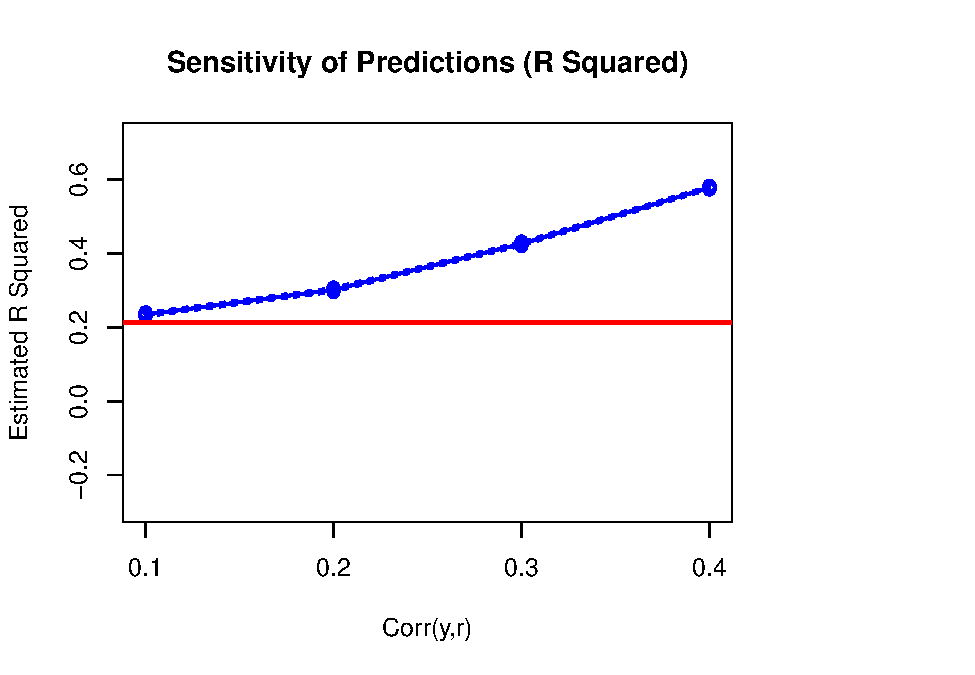
\includegraphics{robustness_checks_files/figure-latex/unnamed-chunk-9-1.pdf}

\hypertarget{bart-with-all-the-predictors}{%
\subsection{BART with all the
predictors}\label{bart-with-all-the-predictors}}

Let's now build a first BART model with all the predictors.

\begin{Shaded}
\begin{Highlighting}[]
\NormalTok{predictors <-}\StringTok{ }\KeywordTok{c}\NormalTok{(}\StringTok{"iso"}\NormalTok{, }\StringTok{"tfp_acf"}\NormalTok{, }\StringTok{"Number_of_patents"}\NormalTok{, }
                \StringTok{"Number_of_trademarks"}\NormalTok{, }\StringTok{"consdummy"}\NormalTok{, }
                \StringTok{"control"}\NormalTok{,}\StringTok{"nace_2"}\NormalTok{, }\StringTok{"fin_rev"}\NormalTok{, }\StringTok{"int_paid"}\NormalTok{,}
                \StringTok{"ebitda"}\NormalTok{, }\StringTok{"cash_flow"}\NormalTok{, }\StringTok{"depr"}\NormalTok{, }\StringTok{"revenue"}\NormalTok{,}
                \StringTok{"total_assets"}\NormalTok{, }\StringTok{"long_term_debt"}\NormalTok{, }\StringTok{"employees"}\NormalTok{,}
                \StringTok{"added_value"}\NormalTok{, }\StringTok{"materials"}\NormalTok{, }\StringTok{"wage_bill"}\NormalTok{, }\StringTok{"loans"}\NormalTok{ ,}
                \StringTok{"int_fixed_assets"}\NormalTok{,}\StringTok{"fixed_assets"}\NormalTok{, }\StringTok{"current_liabilities"}\NormalTok{,}
                \StringTok{"liquidity_ratio"}\NormalTok{,  }\StringTok{"solvency_ratio"}\NormalTok{, }\StringTok{"current_assets"}\NormalTok{,}
                \StringTok{"fin_expenses"}\NormalTok{, }\StringTok{"net_income"}\NormalTok{,  }\StringTok{"fin_cons100"}\NormalTok{ , }\StringTok{"inv"}\NormalTok{ ,}
                \StringTok{"real_SA"}\NormalTok{, }\StringTok{"shareholders_funds"}\NormalTok{ , }\StringTok{"NEG_VA"}\NormalTok{ ,}\StringTok{"ICR_failure"}\NormalTok{ ,}
                \StringTok{"profitability"}\NormalTok{ ,  }\StringTok{"misallocated_fixed"}\NormalTok{ , }\StringTok{"interest_diff"}\NormalTok{) }
\CommentTok{# , "+ capital_intensity", "labour_product"}
\NormalTok{dati}\OperatorTok{$}\NormalTok{X <-}\KeywordTok{as.data.frame}\NormalTok{(dati[predictors])}
\end{Highlighting}
\end{Shaded}

\begin{Shaded}
\begin{Highlighting}[]
\KeywordTok{set.seed}\NormalTok{(}\DecValTok{123}\NormalTok{)}
\KeywordTok{system.time}\NormalTok{(\{}
\NormalTok{bart_predictors<-}\KeywordTok{bartMachine}\NormalTok{(dati}\OperatorTok{$}\NormalTok{X,}\KeywordTok{as.factor}\NormalTok{(dati}\OperatorTok{$}\NormalTok{failure), }\DataTypeTok{use_missing_data=}\OtherTok{TRUE}\NormalTok{) }
\NormalTok{\})}

\NormalTok{dati}\OperatorTok{$}\NormalTok{fitted.results.bart.predictors <-}\StringTok{ }\DecValTok{1}\OperatorTok{-}\StringTok{ }\KeywordTok{round}\NormalTok{(}\KeywordTok{predict}\NormalTok{(bart_predictors, dati}\OperatorTok{$}\NormalTok{X,}
                                                        \DataTypeTok{type=}\StringTok{'prob'}\NormalTok{), }\DecValTok{6}\NormalTok{)}
\NormalTok{dati}\OperatorTok{$}\NormalTok{fitted.results.bart.predictors <-}\StringTok{ }\KeywordTok{as.numeric}\NormalTok{(dati}\OperatorTok{$}\NormalTok{fitted.results.bart.predictors)}
\NormalTok{predictions <-}\StringTok{ }\KeywordTok{as.data.frame}\NormalTok{(}\KeywordTok{cbind}\NormalTok{(dati}\OperatorTok{$}\NormalTok{id, dati}\OperatorTok{$}\NormalTok{fitted.results.bart.predictors))}
\end{Highlighting}
\end{Shaded}

\textit{Negative Added Value} results to be the best predictor in the
model.

\begin{Shaded}
\begin{Highlighting}[]
\KeywordTok{investigate_var_importance}\NormalTok{(bart_predictors, }\DataTypeTok{num_replicates_for_avg =} \DecValTok{20}\NormalTok{) }
\end{Highlighting}
\end{Shaded}

\begin{verbatim}
## ....................
\end{verbatim}

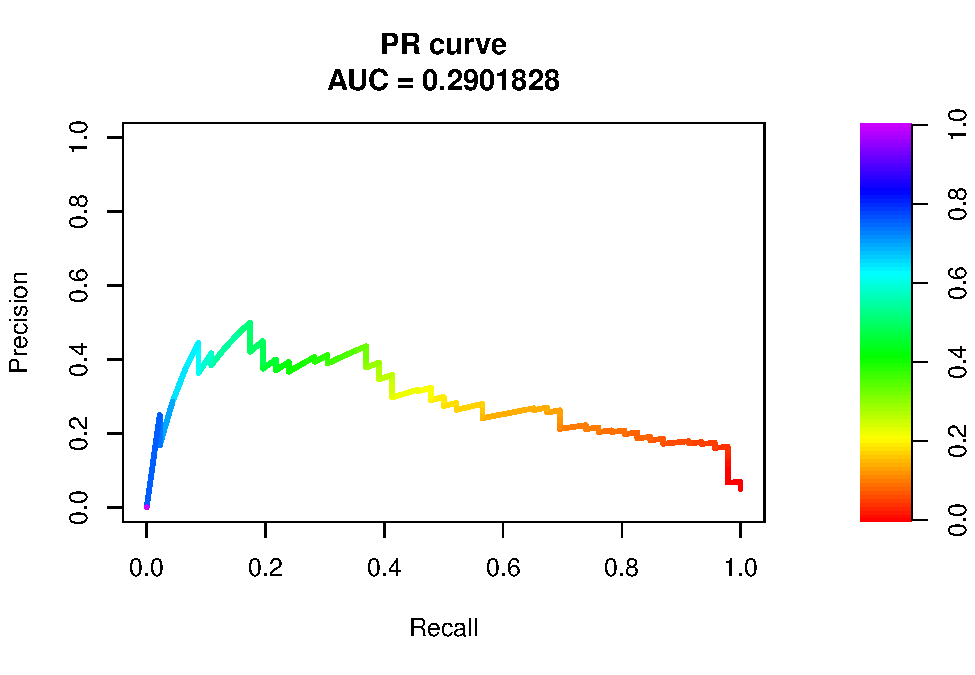
\includegraphics{robustness_checks_files/figure-latex/unnamed-chunk-12-1.pdf}

Generate the matrix of predictors with the new predictor that we
generated before \(R_i\) (\textit{robust}).

\begin{Shaded}
\begin{Highlighting}[]
\NormalTok{robust <-}\StringTok{ }\KeywordTok{c}\NormalTok{(}\StringTok{"iso"}\NormalTok{, }\StringTok{"tfp_acf"}\NormalTok{, }\StringTok{"Number_of_patents"}\NormalTok{, }\StringTok{"Number_of_trademarks"}\NormalTok{,}
  \StringTok{"consdummy"}\NormalTok{, }\StringTok{"control"}\NormalTok{,}\StringTok{"nace_2"}\NormalTok{, }\StringTok{"fin_rev"}\NormalTok{, }\StringTok{"int_paid"}\NormalTok{, }\StringTok{"ebitda"}\NormalTok{, }\StringTok{"cash_flow"}\NormalTok{,}
  \StringTok{"depr"}\NormalTok{, }\StringTok{"revenue"}\NormalTok{, }\StringTok{"total_assets"}\NormalTok{, }\StringTok{"long_term_debt"}\NormalTok{, }\StringTok{"employees"}\NormalTok{, }\StringTok{"added_value"}\NormalTok{,}
  \StringTok{"materials"}\NormalTok{, }\StringTok{"wage_bill"}\NormalTok{, }\StringTok{"loans"}\NormalTok{ , }\StringTok{"int_fixed_assets"}\NormalTok{,}\StringTok{"fixed_assets"}\NormalTok{,}
  \StringTok{"current_liabilities"}\NormalTok{,  }\StringTok{"liquidity_ratio"}\NormalTok{,  }\StringTok{"solvency_ratio"}\NormalTok{, }\StringTok{"current_assets"}\NormalTok{,}
  \StringTok{"fin_expenses"}\NormalTok{, }\StringTok{"net_income"}\NormalTok{,  }\StringTok{"fin_cons100"}\NormalTok{ , }\StringTok{"inv"}\NormalTok{ , }\StringTok{"real_SA"}\NormalTok{, }\StringTok{"shareholders_funds"}\NormalTok{ ,}
  \StringTok{"NEG_VA"}\NormalTok{ ,}\StringTok{"ICR_failure"}\NormalTok{ , }\StringTok{"profitability"}\NormalTok{ ,  }\StringTok{"misallocated_fixed"}\NormalTok{ , }\StringTok{"interest_diff"}\NormalTok{ ,}
  \StringTok{"robust"}\NormalTok{)}
\end{Highlighting}
\end{Shaded}

\hypertarget{create-the-bart-function}{%
\subsection{Create the BART function}\label{create-the-bart-function}}

We now create a BART function that will run on different boostraped
samples.

\begin{Shaded}
\begin{Highlighting}[]
\NormalTok{bart <-}\StringTok{ }\ControlFlowTok{function}\NormalTok{(sample) \{}
\NormalTok{  bart_machine<-}\StringTok{ }\KeywordTok{bartMachine}\NormalTok{(X, Y,}
  \DataTypeTok{use_missing_data=}\OtherTok{TRUE}\NormalTok{)}
\NormalTok{  sample}\OperatorTok{$}\NormalTok{fitted.results.bart <-}\StringTok{ }\DecValTok{1}\OperatorTok{-}\StringTok{ }\KeywordTok{round}\NormalTok{(}\KeywordTok{predict}\NormalTok{(bart_machine, X,  }\DataTypeTok{type=}\StringTok{'prob'}\NormalTok{), }\DecValTok{6}\NormalTok{)}
\NormalTok{  res <-}\StringTok{ }\KeywordTok{cbind}\NormalTok{(sample}\OperatorTok{$}\NormalTok{id, sample}\OperatorTok{$}\NormalTok{fitted.results.bart)}
  \KeywordTok{return}\NormalTok{(res)}
\NormalTok{\}}
\end{Highlighting}
\end{Shaded}

\hypertarget{robustness-check-what-happens-when-we-introduce-a-new-strong-predictor-1}{%
\section{Robustness check: what happens when we introduce a new
``strong'' predictor?
(1)}\label{robustness-check-what-happens-when-we-introduce-a-new-strong-predictor-1}}

Let's first see how many times the predictions of the first BART
(without \(R_i\)) are contained in the confindence intervals of the
predictions build for \(\hat{p}(Y_i = 1 |X_i = x, R_i = r)\).

\begin{Shaded}
\begin{Highlighting}[]
\NormalTok{### Create matrix to save bootstrapped results (N = B)}
\NormalTok{B=}\DecValTok{6}
\NormalTok{results<-}\KeywordTok{matrix}\NormalTok{(}\DataTypeTok{data=}\OtherTok{NA}\NormalTok{, }\DataTypeTok{nrow =} \KeywordTok{nrow}\NormalTok{(dati)}\OperatorTok{*}\FloatTok{0.95}\NormalTok{, }\DataTypeTok{ncol =}\NormalTok{ B)}
\NormalTok{id<-}\KeywordTok{matrix}\NormalTok{(}\DataTypeTok{data=}\OtherTok{NA}\NormalTok{, }\DataTypeTok{nrow =} \KeywordTok{nrow}\NormalTok{(dati)}\OperatorTok{*}\FloatTok{0.95}\NormalTok{, }\DataTypeTok{ncol =}\NormalTok{ B)}
\NormalTok{merge <-}\StringTok{ }\KeywordTok{matrix}\NormalTok{(}\DataTypeTok{data=}\OtherTok{NA}\NormalTok{, }\DataTypeTok{nrow =} \KeywordTok{nrow}\NormalTok{(dati)}\OperatorTok{*}\FloatTok{0.95}\NormalTok{, }\DataTypeTok{ncol =}\NormalTok{ B}\OperatorTok{*}\DecValTok{2}\NormalTok{)}

\CommentTok{#prob1 <- rep(1/nrow(dati), nrow(dati))}
\CommentTok{#prob1}

\NormalTok{### Start loop}
\KeywordTok{set.seed}\NormalTok{(}\DecValTok{123}\NormalTok{)}
\ControlFlowTok{for}\NormalTok{ (i }\ControlFlowTok{in}\NormalTok{ (}\DecValTok{1}\OperatorTok{:}\NormalTok{B)) \{}
  \CommentTok{# Repeatedly (B) draw subsamples}
\NormalTok{  sample <-}\StringTok{ }\NormalTok{dati[}\KeywordTok{sample}\NormalTok{(}\DecValTok{1}\OperatorTok{:}\KeywordTok{nrow}\NormalTok{(dati), }\KeywordTok{nrow}\NormalTok{(dati)}\OperatorTok{*}\FloatTok{0.95}\NormalTok{, }\DataTypeTok{replace =} \OtherTok{FALSE}\NormalTok{),]}
  
\NormalTok{  X <-}\KeywordTok{as.data.frame}\NormalTok{(sample[robust]) }
\NormalTok{  Y <-}\StringTok{ }\KeywordTok{as.factor}\NormalTok{(sample}\OperatorTok{$}\NormalTok{failure)}
  
  \CommentTok{# split into training and test }
  \CommentTok{#train_ind <- sample(seq_len(nrow(dati)), size = nrow(dati)*0.9) }
  \CommentTok{#train <- dati[train_ind,]}
  \CommentTok{#test <-  dati[-train_ind,]}
  
  \CommentTok{#BART}
\NormalTok{  merge[, ((i}\OperatorTok{*}\DecValTok{2}\NormalTok{)}\OperatorTok{-}\DecValTok{1}\NormalTok{)}\OperatorTok{:}\NormalTok{(i}\OperatorTok{*}\DecValTok{2}\NormalTok{)] <-}\StringTok{ }\KeywordTok{bart}\NormalTok{(sample)}
\NormalTok{  id[,i]  <-}\StringTok{ }\NormalTok{merge[,((i}\OperatorTok{*}\DecValTok{2}\NormalTok{)}\OperatorTok{-}\DecValTok{1}\NormalTok{)]}
\NormalTok{  results[,i] <-}\StringTok{ }\NormalTok{merge[,(i}\OperatorTok{*}\DecValTok{2}\NormalTok{)]}
  \CommentTok{#merge[, ((i*2)-1):(i*2)] <- cbind(id[,i], results[,i])}
\NormalTok{\}}
\end{Highlighting}
\end{Shaded}

\begin{Shaded}
\begin{Highlighting}[]
\CommentTok{# The following code is for the predictions of the "Robust model"}
\KeywordTok{length}\NormalTok{(}\KeywordTok{unique}\NormalTok{(dati}\OperatorTok{$}\NormalTok{id))}
\KeywordTok{length}\NormalTok{(}\KeywordTok{unique}\NormalTok{(id[,}\DecValTok{1}\NormalTok{])) }\CommentTok{#which are the unique IDs?}

\CommentTok{# Overlapping observations between the different samples}
\CommentTok{# Namely, obs that are drawn in all the samples}
\NormalTok{bootstrap <-}\StringTok{ }\KeywordTok{as.data.frame}\NormalTok{(id[,}\DecValTok{1}\NormalTok{][id[,}\DecValTok{1}\NormalTok{] }\OperatorTok\StringTok{ }\NormalTok{id[,}\DecValTok{2}\NormalTok{]]) }

\ControlFlowTok{for}\NormalTok{ (i }\ControlFlowTok{in}\NormalTok{ (}\DecValTok{3}\OperatorTok{:}\NormalTok{(B))) \{}
\NormalTok{  bootstrap <-}\StringTok{ }\KeywordTok{as.matrix}\NormalTok{(bootstrap[,}\DecValTok{1}\NormalTok{][bootstrap[,}\DecValTok{1}\NormalTok{] }\OperatorTok\StringTok{ }\NormalTok{id[,i]])}
\NormalTok{\}}

\NormalTok{bootstrap <-}\StringTok{ }\KeywordTok{as.data.frame}\NormalTok{(bootstrap)}
\KeywordTok{names}\NormalTok{(bootstrap) <-}\StringTok{ }\KeywordTok{c}\NormalTok{(}\StringTok{"id"}\NormalTok{) }\CommentTok{# IDs of overlapping obs}

\NormalTok{data_merge <-}\StringTok{ }\KeywordTok{as.data.frame}\NormalTok{(merge)}
\KeywordTok{names}\NormalTok{(data_merge) <-}\StringTok{ }\KeywordTok{c}\NormalTok{(}\StringTok{"id"}\NormalTok{, }\StringTok{"values"}\NormalTok{,}
                       \StringTok{"id"}\NormalTok{, }\StringTok{"values"}\NormalTok{,}
                       \StringTok{"id"}\NormalTok{, }\StringTok{"values"}\NormalTok{,}
                       \StringTok{"id"}\NormalTok{, }\StringTok{"values"}\NormalTok{,}
                       \StringTok{"id"}\NormalTok{, }\StringTok{"values"}\NormalTok{,}
                       \StringTok{"id"}\NormalTok{, }\StringTok{"values"}\NormalTok{)}

\CommentTok{# Obtaining the predicted probabilities just for the overlapping IDs}
\NormalTok{total <-}\StringTok{ }\KeywordTok{merge}\NormalTok{(bootstrap,data_merge[,}\DecValTok{1}\OperatorTok{:}\DecValTok{2}\NormalTok{], }\DataTypeTok{by=} \KeywordTok{c}\NormalTok{(}\StringTok{"id"}\NormalTok{))}

\ControlFlowTok{for}\NormalTok{ (i }\ControlFlowTok{in}\NormalTok{ (}\DecValTok{2}\OperatorTok{:}\NormalTok{(B))) \{}
\NormalTok{  total <-}\StringTok{ }\KeywordTok{merge}\NormalTok{(total,data_merge[,((i}\OperatorTok{*}\DecValTok{2}\NormalTok{)}\OperatorTok{-}\DecValTok{1}\NormalTok{)}\OperatorTok{:}\NormalTok{(i}\OperatorTok{*}\DecValTok{2}\NormalTok{)], }\DataTypeTok{by=} \KeywordTok{c}\NormalTok{(}\StringTok{"id"}\NormalTok{))}
\NormalTok{\}}
\NormalTok{total <-}\StringTok{ }\KeywordTok{as.matrix}\NormalTok{(total)}

\CommentTok{# Computing means and SDs of overlapping probabilities}
\NormalTok{tot <-}\StringTok{ }\KeywordTok{matrix}\NormalTok{(}\DataTypeTok{data=}\OtherTok{NA}\NormalTok{, }\DataTypeTok{nrow =} \KeywordTok{nrow}\NormalTok{(total), }\DataTypeTok{ncol =}\NormalTok{ (}\KeywordTok{ncol}\NormalTok{(total)}\OperatorTok{-}\DecValTok{1}\NormalTok{))}
\NormalTok{tot[,}\DecValTok{1}\OperatorTok{:}\NormalTok{(}\KeywordTok{ncol}\NormalTok{(total)}\OperatorTok{-}\DecValTok{1}\NormalTok{)]<-}\KeywordTok{as.matrix}\NormalTok{(}\KeywordTok{sapply}\NormalTok{(total[,}\DecValTok{2}\OperatorTok{:}\KeywordTok{ncol}\NormalTok{(total)], as.numeric))}
\NormalTok{mean_sd<-}\KeywordTok{cbind}\NormalTok{(}\KeywordTok{rowMeans}\NormalTok{(tot[,}\DecValTok{1}\OperatorTok{:}\KeywordTok{ncol}\NormalTok{(tot)]), }\KeywordTok{rowSds}\NormalTok{(tot[,}\DecValTok{1}\OperatorTok{:}\KeywordTok{ncol}\NormalTok{(tot)]))}

\NormalTok{mean_sd <-}\StringTok{ }\KeywordTok{as.data.frame}\NormalTok{(}\KeywordTok{cbind}\NormalTok{(total[,}\DecValTok{1}\NormalTok{], mean_sd[,}\DecValTok{1}\OperatorTok{:}\DecValTok{2}\NormalTok{]))}
\KeywordTok{names}\NormalTok{(mean_sd) <-}\StringTok{ }\KeywordTok{c}\NormalTok{(}\StringTok{"id"}\NormalTok{, }\StringTok{"mean"}\NormalTok{, }\StringTok{"sd"}\NormalTok{)}
\KeywordTok{names}\NormalTok{(predictions) <-}\StringTok{ }\KeywordTok{c}\NormalTok{(}\StringTok{"id"}\NormalTok{, }\StringTok{"values"}\NormalTok{)}

\CommentTok{# Getting a matrix with means and sd of predicted probabilites}
\CommentTok{# from the "robust" model and the point estimates from the "general" model}
\NormalTok{final <-}\StringTok{ }\KeywordTok{as.data.frame}\NormalTok{(}\KeywordTok{merge}\NormalTok{(mean_sd, predictions, }\DataTypeTok{by=} \KeywordTok{c}\NormalTok{(}\StringTok{"id"}\NormalTok{)))}
\NormalTok{fin <-}\StringTok{ }\KeywordTok{matrix}\NormalTok{(}\DataTypeTok{data=}\OtherTok{NA}\NormalTok{, }\DataTypeTok{nrow =} \KeywordTok{nrow}\NormalTok{(final), }\DataTypeTok{ncol =} \DecValTok{3}\NormalTok{)}
\NormalTok{fin[,}\DecValTok{1}\OperatorTok{:}\DecValTok{3}\NormalTok{]<-}\StringTok{ }\KeywordTok{as.matrix}\NormalTok{(}\KeywordTok{sapply}\NormalTok{(}\KeywordTok{as.matrix}\NormalTok{(final[,}\DecValTok{2}\OperatorTok{:}\DecValTok{4}\NormalTok{]), as.numeric))}
\NormalTok{fin <-}\StringTok{ }\KeywordTok{as.data.frame}\NormalTok{(fin)}
\KeywordTok{names}\NormalTok{(fin) <-}\StringTok{ }\KeywordTok{c}\NormalTok{(}\StringTok{"mean"}\NormalTok{, }\StringTok{"sd"}\NormalTok{, }\StringTok{"value"}\NormalTok{)}
\end{Highlighting}
\end{Shaded}

The proportion of inclusion of \(\hat{p}(Y_i | X_i = x)\) in the
confidence intervals of \(\hat{p}(Y_i | X_i = x, R_i = r)\) is the
following.

\begin{Shaded}
\begin{Highlighting}[]
\CommentTok{#Change the t-value accordingly to B and alpha}
\KeywordTok{length}\NormalTok{(}\KeywordTok{which}\NormalTok{(fin}\OperatorTok{$}\NormalTok{value }\OperatorTok{<=}\StringTok{ }\NormalTok{(fin}\OperatorTok{$}\NormalTok{mean }\OperatorTok{+}\StringTok{ }\FloatTok{4.03}\OperatorTok{*}\NormalTok{(fin}\OperatorTok{$}\NormalTok{sd}\OperatorTok{/}\KeywordTok{sqrt}\NormalTok{(B))) }\OperatorTok{&}
\NormalTok{fin}\OperatorTok{$}\NormalTok{value }\OperatorTok{>=}\StringTok{ }\NormalTok{(fin}\OperatorTok{$}\NormalTok{mean }\OperatorTok{-}\StringTok{ }\FloatTok{4.03}\OperatorTok{*}\NormalTok{(fin}\OperatorTok{$}\NormalTok{sd}\OperatorTok{/}\KeywordTok{sqrt}\NormalTok{(B))) ))}\OperatorTok{/}\KeywordTok{nrow}\NormalTok{(fin)}
\end{Highlighting}
\end{Shaded}

\begin{verbatim}
## [1] 0.5408654
\end{verbatim}

\hypertarget{robustness-check-what-happens-when-we-introduce-a-new-strong-predictor-2}{%
\section{Robustness check: what happens when we introduce a new
``strong'' predictor?
(2)}\label{robustness-check-what-happens-when-we-introduce-a-new-strong-predictor-2}}

\hypertarget{check-of-ci-overlap}{%
\subsection{Check of CI overlap}\label{check-of-ci-overlap}}

This time we perform a bootstrap with replacement also for the general
model (the one without \(R_i\)) and we will see how large is the overlap
between the confidence intervals of the predictions of
\(\hat{p}_i(Y_i = 1 | X_i = x)\) and
\(\hat{p}_i(Y_i = 1 | X_i = x, R_i = r)\).

\hypertarget{robust-model}{%
\subsection{Robust Model}\label{robust-model}}

\begin{Shaded}
\begin{Highlighting}[]
\NormalTok{### Create matrix to save bootstrapped results (N = B)}
\NormalTok{B=}\DecValTok{4}
\NormalTok{results<-}\KeywordTok{matrix}\NormalTok{(}\DataTypeTok{data=}\OtherTok{NA}\NormalTok{, }\DataTypeTok{nrow =} \KeywordTok{nrow}\NormalTok{(dati), }\DataTypeTok{ncol =}\NormalTok{ B)}
\NormalTok{id<-}\KeywordTok{matrix}\NormalTok{(}\DataTypeTok{data=}\OtherTok{NA}\NormalTok{, }\DataTypeTok{nrow =} \KeywordTok{nrow}\NormalTok{(dati), }\DataTypeTok{ncol =}\NormalTok{ B)}
\NormalTok{merge <-}\StringTok{ }\KeywordTok{matrix}\NormalTok{(}\DataTypeTok{data=}\OtherTok{NA}\NormalTok{, }\DataTypeTok{nrow =} \KeywordTok{nrow}\NormalTok{(dati), }\DataTypeTok{ncol =}\NormalTok{ B}\OperatorTok{*}\DecValTok{2}\NormalTok{)}

\CommentTok{#prob1 <- rep(1/nrow(dati), nrow(dati))}
\CommentTok{#prob1}

\NormalTok{### Start loop for ROBUST}

\ControlFlowTok{for}\NormalTok{ (i }\ControlFlowTok{in}\NormalTok{ (}\DecValTok{1}\OperatorTok{:}\NormalTok{B)) \{}
  \KeywordTok{set.seed}\NormalTok{(}\DecValTok{123} \OperatorTok{+}\StringTok{ }\NormalTok{i)}
  \CommentTok{# Repeatedly (B) draw subsamples}
\NormalTok{  sample <-}\StringTok{ }\NormalTok{dati[}\KeywordTok{sample}\NormalTok{(}\DecValTok{1}\OperatorTok{:}\KeywordTok{nrow}\NormalTok{(dati), }\KeywordTok{nrow}\NormalTok{(dati), }\DataTypeTok{replace =} \OtherTok{TRUE}\NormalTok{),]}
  
\NormalTok{  X <-}\KeywordTok{as.data.frame}\NormalTok{(sample[robust]) }
\NormalTok{  Y <-}\StringTok{ }\KeywordTok{as.factor}\NormalTok{(sample}\OperatorTok{$}\NormalTok{failure)}
  
  \CommentTok{# split into training and test }
  \CommentTok{#train_ind <- sample(seq_len(nrow(dati)), size = nrow(dati)*0.9) }
  \CommentTok{#train <- dati[train_ind,]}
  \CommentTok{#test <-  dati[-train_ind,]}
  
  \CommentTok{#BART}
\NormalTok{  merge[, ((i}\OperatorTok{*}\DecValTok{2}\NormalTok{)}\OperatorTok{-}\DecValTok{1}\NormalTok{)}\OperatorTok{:}\NormalTok{(i}\OperatorTok{*}\DecValTok{2}\NormalTok{)] <-}\StringTok{ }\KeywordTok{bart}\NormalTok{(sample)}
\NormalTok{  id[,i]  <-}\StringTok{ }\NormalTok{merge[,((i}\OperatorTok{*}\DecValTok{2}\NormalTok{)}\OperatorTok{-}\DecValTok{1}\NormalTok{)]}
\NormalTok{  results[,i] <-}\StringTok{ }\NormalTok{merge[,(i}\OperatorTok{*}\DecValTok{2}\NormalTok{)]}
  \CommentTok{#merge[, ((i*2)-1):(i*2)] <- cbind(id[,i], results[,i])}
\NormalTok{\}}
\end{Highlighting}
\end{Shaded}

\begin{Shaded}
\begin{Highlighting}[]
\CommentTok{# The comments are the same of the previous chunk}

\CommentTok{# The following code is for the model "robust"}
\KeywordTok{length}\NormalTok{(}\KeywordTok{unique}\NormalTok{(dati}\OperatorTok{$}\NormalTok{id))}
\KeywordTok{length}\NormalTok{(}\KeywordTok{unique}\NormalTok{(id[,}\DecValTok{1}\NormalTok{]))}
\NormalTok{bootstrap <-}\StringTok{ }\KeywordTok{as.data.frame}\NormalTok{(id[,}\DecValTok{1}\NormalTok{][id[,}\DecValTok{1}\NormalTok{] }\OperatorTok\StringTok{ }\NormalTok{id[,}\DecValTok{2}\NormalTok{]])}

\ControlFlowTok{for}\NormalTok{ (i }\ControlFlowTok{in}\NormalTok{ (}\DecValTok{3}\OperatorTok{:}\NormalTok{(B))) \{}
\NormalTok{  bootstrap <-}\StringTok{ }\KeywordTok{as.matrix}\NormalTok{(bootstrap[,}\DecValTok{1}\NormalTok{][bootstrap[,}\DecValTok{1}\NormalTok{] }\OperatorTok\StringTok{ }\NormalTok{id[,i]])}
\NormalTok{\}}

\NormalTok{bootstrap <-}\StringTok{ }\KeywordTok{as.data.frame}\NormalTok{(bootstrap)}
\KeywordTok{names}\NormalTok{(bootstrap) <-}\StringTok{ }\KeywordTok{c}\NormalTok{(}\StringTok{"id"}\NormalTok{)}

\NormalTok{data_merge <-}\StringTok{ }\KeywordTok{as.data.frame}\NormalTok{(merge)}
\KeywordTok{names}\NormalTok{(data_merge) <-}\StringTok{ }\KeywordTok{c}\NormalTok{(}\StringTok{"id"}\NormalTok{, }\StringTok{"values"}\NormalTok{,}
                       \StringTok{"id"}\NormalTok{, }\StringTok{"values"}\NormalTok{,}
                       \StringTok{"id"}\NormalTok{, }\StringTok{"values"}\NormalTok{,}
                       \StringTok{"id"}\NormalTok{, }\StringTok{"values"}\NormalTok{) }\CommentTok{#change accordingly}

\NormalTok{total <-}\StringTok{ }\KeywordTok{merge}\NormalTok{(bootstrap,data_merge[,}\DecValTok{1}\OperatorTok{:}\DecValTok{2}\NormalTok{], }\DataTypeTok{by=} \KeywordTok{c}\NormalTok{(}\StringTok{"id"}\NormalTok{))}

\ControlFlowTok{for}\NormalTok{ (i }\ControlFlowTok{in}\NormalTok{ (}\DecValTok{2}\OperatorTok{:}\NormalTok{(B))) \{}
\NormalTok{  total <-}\StringTok{ }\KeywordTok{merge}\NormalTok{(total,data_merge[,((i}\OperatorTok{*}\DecValTok{2}\NormalTok{)}\OperatorTok{-}\DecValTok{1}\NormalTok{)}\OperatorTok{:}\NormalTok{(i}\OperatorTok{*}\DecValTok{2}\NormalTok{)], }\DataTypeTok{by=} \KeywordTok{c}\NormalTok{(}\StringTok{"id"}\NormalTok{))}
\NormalTok{\}}

\NormalTok{total <-}\StringTok{ }\KeywordTok{as.matrix}\NormalTok{(total)}

\KeywordTok{library}\NormalTok{(matrixStats)}
\NormalTok{tot <-}\StringTok{ }\KeywordTok{matrix}\NormalTok{(}\DataTypeTok{data=}\OtherTok{NA}\NormalTok{, }\DataTypeTok{nrow =} \KeywordTok{nrow}\NormalTok{(total), }\DataTypeTok{ncol =}\NormalTok{ (}\KeywordTok{ncol}\NormalTok{(total)}\OperatorTok{-}\DecValTok{1}\NormalTok{))}
\NormalTok{tot[,}\DecValTok{1}\OperatorTok{:}\NormalTok{(}\KeywordTok{ncol}\NormalTok{(total)}\OperatorTok{-}\DecValTok{1}\NormalTok{)]<-}\KeywordTok{as.matrix}\NormalTok{(}\KeywordTok{sapply}\NormalTok{(total[,}\DecValTok{2}\OperatorTok{:}\KeywordTok{ncol}\NormalTok{(total)], as.numeric))}
\NormalTok{mean_sd<-}\KeywordTok{cbind}\NormalTok{(}\KeywordTok{rowMeans}\NormalTok{(tot[,}\DecValTok{1}\OperatorTok{:}\KeywordTok{ncol}\NormalTok{(tot)]), }\KeywordTok{rowSds}\NormalTok{(tot[,}\DecValTok{1}\OperatorTok{:}\KeywordTok{ncol}\NormalTok{(tot)]))}

\NormalTok{mean_sd <-}\StringTok{ }\KeywordTok{as.data.frame}\NormalTok{(}\KeywordTok{cbind}\NormalTok{(total[,}\DecValTok{1}\NormalTok{], mean_sd[,}\DecValTok{1}\OperatorTok{:}\DecValTok{2}\NormalTok{]))}
\KeywordTok{names}\NormalTok{(mean_sd) <-}\StringTok{ }\KeywordTok{c}\NormalTok{(}\StringTok{"id"}\NormalTok{, }\StringTok{"mean"}\NormalTok{, }\StringTok{"sd"}\NormalTok{)}
\end{Highlighting}
\end{Shaded}

\begin{Shaded}
\begin{Highlighting}[]
\CommentTok{# Matrix for the Mean and SD of the predicted probabilities}
\KeywordTok{length}\NormalTok{(}\KeywordTok{unique}\NormalTok{(mean_sd}\OperatorTok{$}\NormalTok{id))}
\end{Highlighting}
\end{Shaded}

\begin{verbatim}
## [1] 738
\end{verbatim}

\begin{Shaded}
\begin{Highlighting}[]
\NormalTok{mean_sd <-}\StringTok{ }\KeywordTok{subset}\NormalTok{(mean_sd, }\OperatorTok{!}\KeywordTok{duplicated}\NormalTok{(mean_sd}\OperatorTok{$}\NormalTok{id))}
\KeywordTok{head}\NormalTok{(mean_sd)}
\end{Highlighting}
\end{Shaded}

\begin{verbatim}
##             id                 mean                   sd
## 1  ESA01016120 3.45000000000207e-05 5.82208439192385e-05
## 3  ESA08240095  0.00620349999999998  0.00844694285920456
## 19 ESA08258451              0.09862   0.0508179995867606
## 23 ESA20521498 0.000157249999999998 0.000198813773835351
## 27 ESA28034254           0.18913375    0.061974100915221
## 28 ESA95209037  0.00232874999999999  0.00182647591005195
\end{verbatim}

\hypertarget{general-model}{%
\subsection{General model}\label{general-model}}

\begin{Shaded}
\begin{Highlighting}[]
\NormalTok{results_model<-}\KeywordTok{matrix}\NormalTok{(}\DataTypeTok{data=}\OtherTok{NA}\NormalTok{, }\DataTypeTok{nrow =} \KeywordTok{nrow}\NormalTok{(dati), }\DataTypeTok{ncol =}\NormalTok{ B)}
\NormalTok{id_model<-}\KeywordTok{matrix}\NormalTok{(}\DataTypeTok{data=}\OtherTok{NA}\NormalTok{, }\DataTypeTok{nrow =} \KeywordTok{nrow}\NormalTok{(dati), }\DataTypeTok{ncol =}\NormalTok{ B)}
\NormalTok{merge_model <-}\StringTok{ }\KeywordTok{matrix}\NormalTok{(}\DataTypeTok{data=}\OtherTok{NA}\NormalTok{, }\DataTypeTok{nrow =} \KeywordTok{nrow}\NormalTok{(dati), }\DataTypeTok{ncol =}\NormalTok{ B}\OperatorTok{*}\DecValTok{2}\NormalTok{)}

\CommentTok{# Start Loop}

\ControlFlowTok{for}\NormalTok{ (i }\ControlFlowTok{in}\NormalTok{ (}\DecValTok{1}\OperatorTok{:}\NormalTok{B)) \{}
  \KeywordTok{set.seed}\NormalTok{(}\DecValTok{123} \OperatorTok{+}\StringTok{ }\NormalTok{i)}
  \CommentTok{# Repeatedly (B) draw subsamples}
\NormalTok{  sample <-}\StringTok{ }\NormalTok{dati[}\KeywordTok{sample}\NormalTok{(}\DecValTok{1}\OperatorTok{:}\KeywordTok{nrow}\NormalTok{(dati), }\KeywordTok{nrow}\NormalTok{(dati), }\DataTypeTok{replace =} \OtherTok{TRUE}\NormalTok{),]}
  
\NormalTok{  X <-}\KeywordTok{as.data.frame}\NormalTok{(sample[predictors]) }
\NormalTok{  Y <-}\StringTok{ }\KeywordTok{as.factor}\NormalTok{(sample}\OperatorTok{$}\NormalTok{failure)}
  
  \CommentTok{# split into training and test }
  \CommentTok{#train_ind <- sample(seq_len(nrow(dati)), size = nrow(dati)*0.9) }
  \CommentTok{#train <- dati[train_ind,]}
  \CommentTok{#test <-  dati[-train_ind,]}
  
  \CommentTok{#BART}
\NormalTok{  merge_model[, ((i}\OperatorTok{*}\DecValTok{2}\NormalTok{)}\OperatorTok{-}\DecValTok{1}\NormalTok{)}\OperatorTok{:}\NormalTok{(i}\OperatorTok{*}\DecValTok{2}\NormalTok{)] <-}\StringTok{ }\KeywordTok{bart}\NormalTok{(sample)}
\NormalTok{  id_model[,i]  <-}\StringTok{ }\NormalTok{merge_model[,((i}\OperatorTok{*}\DecValTok{2}\NormalTok{)}\OperatorTok{-}\DecValTok{1}\NormalTok{)]}
\NormalTok{  results_model[,i] <-}\StringTok{ }\NormalTok{merge_model[,(i}\OperatorTok{*}\DecValTok{2}\NormalTok{)]}
  \CommentTok{#merge[, ((i*2)-1):(i*2)] <- cbind(id[,i], results[,i])}
\NormalTok{\}}
\end{Highlighting}
\end{Shaded}

\begin{Shaded}
\begin{Highlighting}[]
\CommentTok{# The comments are the same of the previous chunk}

\CommentTok{# The following code is for the model "general"}
\KeywordTok{length}\NormalTok{(}\KeywordTok{unique}\NormalTok{(id_model[,}\DecValTok{1}\NormalTok{]))}
\NormalTok{bootstrap_model <-}\StringTok{ }\KeywordTok{as.data.frame}\NormalTok{(id_model[,}\DecValTok{1}\NormalTok{][id_model[,}\DecValTok{1}\NormalTok{] }\OperatorTok\StringTok{ }\NormalTok{id_model[,}\DecValTok{2}\NormalTok{]])}

\ControlFlowTok{for}\NormalTok{ (i }\ControlFlowTok{in}\NormalTok{ (}\DecValTok{3}\OperatorTok{:}\NormalTok{(B))) \{}
\NormalTok{  bootstrap_model <-}\StringTok{ }\KeywordTok{as.matrix}\NormalTok{(bootstrap_model[,}\DecValTok{1}\NormalTok{][bootstrap_model[,}\DecValTok{1}\NormalTok{] }\OperatorTok\StringTok{ }\NormalTok{id_model[,i]])}
\NormalTok{\}}

\NormalTok{bootstrap_model <-}\StringTok{ }\KeywordTok{as.data.frame}\NormalTok{(bootstrap_model)}
\KeywordTok{names}\NormalTok{(bootstrap_model) <-}\StringTok{ }\KeywordTok{c}\NormalTok{(}\StringTok{"id"}\NormalTok{)}

\NormalTok{data_merge_model <-}\StringTok{ }\KeywordTok{as.data.frame}\NormalTok{(merge_model)}
\KeywordTok{names}\NormalTok{(data_merge_model) <-}\StringTok{ }\KeywordTok{c}\NormalTok{(}\StringTok{"id"}\NormalTok{, }\StringTok{"values"}\NormalTok{,}
                       \StringTok{"id"}\NormalTok{, }\StringTok{"values"}\NormalTok{,}
                       \StringTok{"id"}\NormalTok{, }\StringTok{"values"}\NormalTok{,}
                       \StringTok{"id"}\NormalTok{, }\StringTok{"values"}\NormalTok{) }\CommentTok{#change accordingly}

\NormalTok{total_model <-}\StringTok{ }\KeywordTok{merge}\NormalTok{(bootstrap_model,data_merge_model[,}\DecValTok{1}\OperatorTok{:}\DecValTok{2}\NormalTok{], }\DataTypeTok{by=} \KeywordTok{c}\NormalTok{(}\StringTok{"id"}\NormalTok{))}

\ControlFlowTok{for}\NormalTok{ (i }\ControlFlowTok{in}\NormalTok{ (}\DecValTok{2}\OperatorTok{:}\NormalTok{(B))) \{}
\NormalTok{  total_model <-}\StringTok{ }\KeywordTok{merge}\NormalTok{(total_model,data_merge_model[,((i}\OperatorTok{*}\DecValTok{2}\NormalTok{)}\OperatorTok{-}\DecValTok{1}\NormalTok{)}\OperatorTok{:}\NormalTok{(i}\OperatorTok{*}\DecValTok{2}\NormalTok{)], }\DataTypeTok{by=} \KeywordTok{c}\NormalTok{(}\StringTok{"id"}\NormalTok{))}
\NormalTok{\}}

\NormalTok{total_model <-}\StringTok{ }\KeywordTok{as.matrix}\NormalTok{(total_model)}

\NormalTok{tot_model <-}\StringTok{ }\KeywordTok{matrix}\NormalTok{(}\DataTypeTok{data=}\OtherTok{NA}\NormalTok{, }\DataTypeTok{nrow =} \KeywordTok{nrow}\NormalTok{(total_model), }\DataTypeTok{ncol =}\NormalTok{ (}\KeywordTok{ncol}\NormalTok{(total_model)}\OperatorTok{-}\DecValTok{1}\NormalTok{))}
\NormalTok{tot_model[,}\DecValTok{1}\OperatorTok{:}\NormalTok{(}\KeywordTok{ncol}\NormalTok{(total_model)}\OperatorTok{-}\DecValTok{1}\NormalTok{)]<-}\KeywordTok{as.matrix}\NormalTok{(}\KeywordTok{sapply}\NormalTok{(total_model[,}\DecValTok{2}\OperatorTok{:}\KeywordTok{ncol}\NormalTok{(total_model)], as.numeric))}
\NormalTok{mean_sd_model<-}\KeywordTok{cbind}\NormalTok{(}\KeywordTok{rowMeans}\NormalTok{(tot_model[,}\DecValTok{1}\OperatorTok{:}\KeywordTok{ncol}\NormalTok{(tot_model)]), }\KeywordTok{rowSds}\NormalTok{(tot_model[,}\DecValTok{1}\OperatorTok{:}\KeywordTok{ncol}\NormalTok{(tot_model)]))}

\NormalTok{mean_sd_model <-}\StringTok{ }\KeywordTok{as.data.frame}\NormalTok{(}\KeywordTok{cbind}\NormalTok{(total_model[,}\DecValTok{1}\NormalTok{], mean_sd_model[,}\DecValTok{1}\OperatorTok{:}\DecValTok{2}\NormalTok{]))}
\KeywordTok{names}\NormalTok{(mean_sd_model) <-}\StringTok{ }\KeywordTok{c}\NormalTok{(}\StringTok{"id"}\NormalTok{, }\StringTok{"mean_model"}\NormalTok{, }\StringTok{"sd_model"}\NormalTok{)}
\end{Highlighting}
\end{Shaded}

\begin{Shaded}
\begin{Highlighting}[]
\CommentTok{# Matrix for the Mean and SD of the predicted probabilities}
\KeywordTok{length}\NormalTok{(}\KeywordTok{unique}\NormalTok{(mean_sd_model}\OperatorTok{$}\NormalTok{id))}
\end{Highlighting}
\end{Shaded}

\begin{verbatim}
## [1] 738
\end{verbatim}

\begin{Shaded}
\begin{Highlighting}[]
\NormalTok{mean_sd_model <-}\StringTok{ }\KeywordTok{subset}\NormalTok{(mean_sd_model, }\OperatorTok{!}\KeywordTok{duplicated}\NormalTok{(mean_sd_model}\OperatorTok{$}\NormalTok{id))}
\KeywordTok{head}\NormalTok{(mean_sd_model)}
\end{Highlighting}
\end{Shaded}

\begin{verbatim}
##             id           mean_model             sd_model
## 1  ESA01016120 4.02499999999917e-05 4.99090840094771e-05
## 3  ESA08240095  0.00155075000000002  0.00193876461954515
## 19 ESA08258451           0.06926025    0.036177451940631
## 23 ESA20521498 4.70000000000192e-05 7.03088424974617e-05
## 27 ESA28034254             0.124761   0.0257599197203718
## 28 ESA95209037           0.01977425   0.0197731076528198
\end{verbatim}

\hypertarget{merging}{%
\subsection{Merging}\label{merging}}

The overlap between the confidence itervals of the predicted
probabilities between the \textit{general} model (without \(R_i\)) and
the \textit{robust} model (with \(R_i\)) is particularly high. The
overlap is reported below.

\begin{Shaded}
\begin{Highlighting}[]
\NormalTok{final <-}\StringTok{ }\KeywordTok{as.data.frame}\NormalTok{(}\KeywordTok{merge}\NormalTok{(mean_sd, mean_sd_model, }\DataTypeTok{by=} \KeywordTok{c}\NormalTok{(}\StringTok{"id"}\NormalTok{)))}

\NormalTok{fin <-}\StringTok{ }\KeywordTok{matrix}\NormalTok{(}\DataTypeTok{data=}\OtherTok{NA}\NormalTok{, }\DataTypeTok{nrow =} \KeywordTok{nrow}\NormalTok{(final), }\DataTypeTok{ncol =} \KeywordTok{ncol}\NormalTok{(final)}\OperatorTok{-}\DecValTok{1}\NormalTok{)}
\NormalTok{fin[,}\DecValTok{1}\OperatorTok{:}\KeywordTok{ncol}\NormalTok{(fin)]<-}\StringTok{ }\KeywordTok{as.matrix}\NormalTok{(}\KeywordTok{sapply}\NormalTok{(}\KeywordTok{as.matrix}\NormalTok{(final[,}\DecValTok{2}\OperatorTok{:}\KeywordTok{ncol}\NormalTok{(final)]), as.numeric))}
\NormalTok{fin <-}\StringTok{ }\KeywordTok{as.data.frame}\NormalTok{(fin)}
\KeywordTok{names}\NormalTok{(fin) <-}\StringTok{ }\KeywordTok{c}\NormalTok{(}\StringTok{"mean"}\NormalTok{, }\StringTok{"sd"}\NormalTok{, }\StringTok{"mean_model"}\NormalTok{, }\StringTok{"sd_model"}\NormalTok{)}

\CommentTok{#Change the t-value accordingly to B and alpha}

\CommentTok{# CI overlap}
\KeywordTok{length}\NormalTok{(}\KeywordTok{which}\NormalTok{((fin}\OperatorTok{$}\NormalTok{mean_model }\OperatorTok{-}\StringTok{ }\FloatTok{4.03}\OperatorTok{*}\NormalTok{(fin}\OperatorTok{$}\NormalTok{sd_model}\OperatorTok{/}\KeywordTok{sqrt}\NormalTok{(B))) }\OperatorTok{<=}\StringTok{ }\NormalTok{(fin}\OperatorTok{$}\NormalTok{mean }\OperatorTok{+}\StringTok{ }\FloatTok{4.03}\OperatorTok{*}\NormalTok{(fin}\OperatorTok{$}\NormalTok{sd}\OperatorTok{/}\KeywordTok{sqrt}\NormalTok{(B))) }\OperatorTok{&}\StringTok{  }\NormalTok{(fin}\OperatorTok{$}\NormalTok{mean_model }\OperatorTok{+}\StringTok{ }\FloatTok{4.03}\OperatorTok{*}\NormalTok{(fin}\OperatorTok{$}\NormalTok{sd_model}\OperatorTok{/}\KeywordTok{sqrt}\NormalTok{(B))) }\OperatorTok{>=}\StringTok{ }\NormalTok{(fin}\OperatorTok{$}\NormalTok{mean }\OperatorTok{-}\StringTok{ }\FloatTok{4.03}\OperatorTok{*}\NormalTok{(fin}\OperatorTok{$}\NormalTok{sd}\OperatorTok{/}\KeywordTok{sqrt}\NormalTok{(B))) ))}\OperatorTok{/}\KeywordTok{nrow}\NormalTok{(fin)}
\end{Highlighting}
\end{Shaded}

\begin{verbatim}
## [1] 0.9837398
\end{verbatim}

\hypertarget{standardized-difference-in-means}{%
\section{Standardized Difference in
Means}\label{standardized-difference-in-means}}

Moreover, the standardized difference in the means between
\(\hat{p}(Y_i =1 |X_i = x)\) and \(\hat{p}(Y_i = 1|X_i = x, R_i = r)\)
is not significant in all the cases.

\begin{Shaded}
\begin{Highlighting}[]
\CommentTok{# Standardized difference in means}
\NormalTok{diff.means <-}\StringTok{ }\NormalTok{fin}\OperatorTok{$}\NormalTok{mean }\OperatorTok{-}\StringTok{ }\NormalTok{fin}\OperatorTok{$}\NormalTok{mean_model}
\NormalTok{standard.diff.means <-}\StringTok{  }\NormalTok{(fin}\OperatorTok{$}\NormalTok{mean }\OperatorTok{-}\StringTok{ }\NormalTok{fin}\OperatorTok{$}\NormalTok{mean_model)}\OperatorTok{/}\KeywordTok{sqrt}\NormalTok{((fin}\OperatorTok{$}\NormalTok{sd}\OperatorTok{^}\DecValTok{2} \OperatorTok{+}\StringTok{ }\NormalTok{fin}\OperatorTok{$}\NormalTok{sd_model}\OperatorTok{^}\DecValTok{2}\NormalTok{)}\OperatorTok{/}\DecValTok{2}\NormalTok{)}

\CommentTok{# 99% CI (t-student distribution)}
\NormalTok{x0 <-}\StringTok{ }\NormalTok{standard.diff.means }\OperatorTok{-}\StringTok{ }\FloatTok{2.58} \OperatorTok{*}\StringTok{ }\CommentTok{# change accordingly to sample size}
\StringTok{  }\NormalTok{(fin}\OperatorTok{$}\NormalTok{mean }\OperatorTok{-}\StringTok{ }\NormalTok{fin}\OperatorTok{$}\NormalTok{mean_model)}\OperatorTok{/}\KeywordTok{sqrt}\NormalTok{((fin}\OperatorTok{$}\NormalTok{sd}\OperatorTok{^}\DecValTok{2} \OperatorTok{+}\StringTok{ }\NormalTok{fin}\OperatorTok{$}\NormalTok{sd_model}\OperatorTok{^}\DecValTok{2}\NormalTok{)}\OperatorTok{/}\DecValTok{2}\NormalTok{) }\CommentTok{#check dimension}
\NormalTok{x1 <-standard.diff.means  }\OperatorTok{+}\StringTok{ }\FloatTok{2.58} \OperatorTok{*}\StringTok{ }\CommentTok{# change accordingly to sample size}
\StringTok{  }\NormalTok{(fin}\OperatorTok{$}\NormalTok{mean }\OperatorTok{-}\StringTok{ }\NormalTok{fin}\OperatorTok{$}\NormalTok{mean_model)}\OperatorTok{/}\KeywordTok{sqrt}\NormalTok{((fin}\OperatorTok{$}\NormalTok{sd}\OperatorTok{^}\DecValTok{2} \OperatorTok{+}\StringTok{ }\NormalTok{fin}\OperatorTok{$}\NormalTok{sd_model}\OperatorTok{^}\DecValTok{2}\NormalTok{)}\OperatorTok{/}\DecValTok{2}\NormalTok{) }\CommentTok{#check dimension}

\NormalTok{(}\KeywordTok{length}\NormalTok{(}\KeywordTok{which}\NormalTok{(x0 }\OperatorTok{>}\StringTok{ }\DecValTok{0} \OperatorTok{&}\StringTok{ }\NormalTok{x1 }\OperatorTok{<}\StringTok{ }\DecValTok{0}\NormalTok{)) }\OperatorTok{+}\StringTok{ }\KeywordTok{length}\NormalTok{(}\KeywordTok{which}\NormalTok{(x0 }\OperatorTok{<}\StringTok{ }\DecValTok{0} \OperatorTok{&}\StringTok{ }\NormalTok{x1 }\OperatorTok{>}\StringTok{ }\DecValTok{0}\NormalTok{)))}\OperatorTok{/}\StringTok{ }\KeywordTok{length}\NormalTok{(x0)}
\end{Highlighting}
\end{Shaded}

\begin{verbatim}
## [1] 1
\end{verbatim}

This can be seen from the plot of the Standardized difference in means
for the probabilities predicted by the two models.

\includegraphics{robustness_checks_files/figure-latex/unnamed-chunk-26-1.pdf}

Moreover, we run multiple t-tests for the predicted values in the
general model and in the robust model. Below we can see the proportion
of observations that are exceeding the standard significativity levels
of \(0.01\) and \(0.05\).

\begin{Shaded}
\begin{Highlighting}[]
\NormalTok{test <-}\StringTok{ }\KeywordTok{as.data.frame}\NormalTok{(}\KeywordTok{cbind}\NormalTok{(total[,}\DecValTok{1}\NormalTok{], tot))}
\KeywordTok{names}\NormalTok{(test) <-}\StringTok{ }\KeywordTok{c}\NormalTok{(}\StringTok{"id"}\NormalTok{, }\StringTok{"v1"}\NormalTok{, }\StringTok{"v2"}\NormalTok{, }\StringTok{"v3"}\NormalTok{, }\StringTok{"v4"}\NormalTok{)}
\NormalTok{test <-}\StringTok{ }\KeywordTok{subset}\NormalTok{(test, }\OperatorTok{!}\KeywordTok{duplicated}\NormalTok{(test}\OperatorTok{$}\NormalTok{id))}

\NormalTok{test_model <-}\StringTok{ }\KeywordTok{as.data.frame}\NormalTok{(}\KeywordTok{cbind}\NormalTok{(total_model[,}\DecValTok{1}\NormalTok{], tot_model))}
\KeywordTok{names}\NormalTok{(test_model) <-}\StringTok{ }\KeywordTok{c}\NormalTok{(}\StringTok{"id"}\NormalTok{, }\StringTok{"m1"}\NormalTok{, }\StringTok{"m2"}\NormalTok{, }\StringTok{"m3"}\NormalTok{, }\StringTok{"m4"}\NormalTok{)}
\NormalTok{test_model <-}\StringTok{ }\KeywordTok{subset}\NormalTok{(test_model, }\OperatorTok{!}\KeywordTok{duplicated}\NormalTok{(test_model}\OperatorTok{$}\NormalTok{id))}

\NormalTok{testing <-}\StringTok{ }\KeywordTok{as.data.frame}\NormalTok{(}\KeywordTok{merge}\NormalTok{(test, test_model, }\DataTypeTok{by=} \KeywordTok{c}\NormalTok{(}\StringTok{"id"}\NormalTok{)))}
\KeywordTok{dim}\NormalTok{(testing)}
\end{Highlighting}
\end{Shaded}

\begin{verbatim}
## [1] 738   9
\end{verbatim}

\begin{Shaded}
\begin{Highlighting}[]
\NormalTok{test <-}\StringTok{ }\KeywordTok{matrix}\NormalTok{(}\DataTypeTok{data =} \OtherTok{NA}\NormalTok{, }\DataTypeTok{ncol =}\NormalTok{ (}\KeywordTok{ncol}\NormalTok{(testing) }\DecValTok{-5}\NormalTok{), }\DataTypeTok{nrow =} \KeywordTok{nrow}\NormalTok{(testing))}
\NormalTok{test[, }\DecValTok{1}\OperatorTok{:}\DecValTok{4}\NormalTok{] <-}\StringTok{ }\KeywordTok{as.matrix}\NormalTok{(}\KeywordTok{sapply}\NormalTok{(}\KeywordTok{as.matrix}\NormalTok{(testing[,}\DecValTok{2}\OperatorTok{:}\DecValTok{5}\NormalTok{]), as.numeric))}
\NormalTok{test_model <-}\StringTok{ }\KeywordTok{matrix}\NormalTok{(}\DataTypeTok{data =} \OtherTok{NA}\NormalTok{, }\DataTypeTok{ncol =}\NormalTok{ (}\KeywordTok{ncol}\NormalTok{(testing) }\DecValTok{-5}\NormalTok{), }\DataTypeTok{nrow =} \KeywordTok{nrow}\NormalTok{(testing))}
\NormalTok{test_model[,}\DecValTok{1}\OperatorTok{:}\DecValTok{4}\NormalTok{] <-}\StringTok{ }\KeywordTok{as.matrix}\NormalTok{(}\KeywordTok{sapply}\NormalTok{(}\KeywordTok{as.matrix}\NormalTok{(testing[,}\DecValTok{6}\OperatorTok{:}\DecValTok{9}\NormalTok{]), as.numeric))}

\NormalTok{pvalue <-}\StringTok{ }\KeywordTok{matrix}\NormalTok{(}\DataTypeTok{data =} \OtherTok{NA}\NormalTok{, }\DataTypeTok{ncol =} \DecValTok{1}\NormalTok{, }\DataTypeTok{nrow =} \KeywordTok{nrow}\NormalTok{(test))}
\NormalTok{N =}\StringTok{ }\KeywordTok{nrow}\NormalTok{(test)}
\ControlFlowTok{for}\NormalTok{ (i }\ControlFlowTok{in}\NormalTok{ (}\DecValTok{1}\OperatorTok{:}\NormalTok{N)) \{}
\NormalTok{    pvalue[i,] <-}\StringTok{ }\KeywordTok{t.test}\NormalTok{(test[i, ], test_model[i,])}\OperatorTok{$}\NormalTok{p.value}
\NormalTok{\}}

\KeywordTok{length}\NormalTok{(}\KeywordTok{which}\NormalTok{(pvalue[,}\DecValTok{1}\NormalTok{]}\OperatorTok{<}\FloatTok{0.01}\NormalTok{))}\OperatorTok{/}\NormalTok{N}
\end{Highlighting}
\end{Shaded}

\begin{verbatim}
## [1] 0.02168022
\end{verbatim}

\begin{Shaded}
\begin{Highlighting}[]
\KeywordTok{length}\NormalTok{(}\KeywordTok{which}\NormalTok{(pvalue[,}\DecValTok{1}\NormalTok{]}\OperatorTok{<}\FloatTok{0.05}\NormalTok{))}\OperatorTok{/}\NormalTok{N}
\end{Highlighting}
\end{Shaded}

\begin{verbatim}
## [1] 0.09620596
\end{verbatim}

\hypertarget{robustness-check-what-happens-when-we-change-the-sample}{%
\section{Robustness check: what happens when we change the
sample?}\label{robustness-check-what-happens-when-we-change-the-sample}}

We propose to use 10 different bootstrap samples (change B to 10 and run
the ``function'' chunks). What we are interested in is the variance of
the different sampling predictions.

\begin{Shaded}
\begin{Highlighting}[]
\NormalTok{B =}\StringTok{ }\DecValTok{10}
\NormalTok{results_model<-}\KeywordTok{matrix}\NormalTok{(}\DataTypeTok{data=}\OtherTok{NA}\NormalTok{, }\DataTypeTok{nrow =} \KeywordTok{nrow}\NormalTok{(dati), }\DataTypeTok{ncol =}\NormalTok{ B)}
\NormalTok{id_model<-}\KeywordTok{matrix}\NormalTok{(}\DataTypeTok{data=}\OtherTok{NA}\NormalTok{, }\DataTypeTok{nrow =} \KeywordTok{nrow}\NormalTok{(dati), }\DataTypeTok{ncol =}\NormalTok{ B)}
\NormalTok{merge_model <-}\StringTok{ }\KeywordTok{matrix}\NormalTok{(}\DataTypeTok{data=}\OtherTok{NA}\NormalTok{, }\DataTypeTok{nrow =} \KeywordTok{nrow}\NormalTok{(dati), }\DataTypeTok{ncol =}\NormalTok{ B}\OperatorTok{*}\DecValTok{2}\NormalTok{)}

\ControlFlowTok{for}\NormalTok{ (i }\ControlFlowTok{in}\NormalTok{ (}\DecValTok{1}\OperatorTok{:}\NormalTok{B)) \{}
  \KeywordTok{set.seed}\NormalTok{(}\DecValTok{123} \OperatorTok{+}\StringTok{ }\NormalTok{i)}
  \CommentTok{# Repeatedly (B) draw subsamples}
\NormalTok{  sample <-}\StringTok{ }\NormalTok{dati[}\KeywordTok{sample}\NormalTok{(}\DecValTok{1}\OperatorTok{:}\KeywordTok{nrow}\NormalTok{(dati), }\KeywordTok{nrow}\NormalTok{(dati), }\DataTypeTok{replace =} \OtherTok{TRUE}\NormalTok{),]}
  
\NormalTok{  X <-}\KeywordTok{as.data.frame}\NormalTok{(sample[predictors]) }
\NormalTok{  Y <-}\StringTok{ }\KeywordTok{as.factor}\NormalTok{(sample}\OperatorTok{$}\NormalTok{failure)}
  
  \CommentTok{# split into training and test }
  \CommentTok{#train_ind <- sample(seq_len(nrow(dati)), size = nrow(dati)*0.9) }
  \CommentTok{#train <- dati[train_ind,]}
  \CommentTok{#test <-  dati[-train_ind,]}
  
  \CommentTok{#BART}
\NormalTok{  merge_model[, ((i}\OperatorTok{*}\DecValTok{2}\NormalTok{)}\OperatorTok{-}\DecValTok{1}\NormalTok{)}\OperatorTok{:}\NormalTok{(i}\OperatorTok{*}\DecValTok{2}\NormalTok{)] <-}\StringTok{ }\KeywordTok{bart}\NormalTok{(sample)}
\NormalTok{  id_model[,i]  <-}\StringTok{ }\NormalTok{merge_model[,((i}\OperatorTok{*}\DecValTok{2}\NormalTok{)}\OperatorTok{-}\DecValTok{1}\NormalTok{)]}
\NormalTok{  results_model[,i] <-}\StringTok{ }\NormalTok{merge_model[,(i}\OperatorTok{*}\DecValTok{2}\NormalTok{)]}
  \CommentTok{#merge[, ((i*2)-1):(i*2)] <- cbind(id[,i], results[,i])}
\NormalTok{\}}
\end{Highlighting}
\end{Shaded}

\begin{Shaded}
\begin{Highlighting}[]
\KeywordTok{length}\NormalTok{(}\KeywordTok{unique}\NormalTok{(id_model[,}\DecValTok{1}\NormalTok{]))}
\end{Highlighting}
\end{Shaded}

\begin{verbatim}
## [1] 2861
\end{verbatim}

\begin{Shaded}
\begin{Highlighting}[]
\NormalTok{bootstrap_model <-}\StringTok{ }\KeywordTok{as.data.frame}\NormalTok{(id_model[,}\DecValTok{1}\NormalTok{][id_model[,}\DecValTok{1}\NormalTok{] }\OperatorTok\StringTok{ }\NormalTok{id_model[,}\DecValTok{2}\NormalTok{]])}

\ControlFlowTok{for}\NormalTok{ (i }\ControlFlowTok{in}\NormalTok{ (}\DecValTok{3}\OperatorTok{:}\NormalTok{(B))) \{}
\NormalTok{  bootstrap_model <-}\StringTok{ }\KeywordTok{as.matrix}\NormalTok{(bootstrap_model[,}\DecValTok{1}\NormalTok{][bootstrap_model[,}\DecValTok{1}\NormalTok{] }\OperatorTok\StringTok{ }\NormalTok{id_model[,i]])}
\NormalTok{\}}

\NormalTok{bootstrap_model <-}\StringTok{ }\KeywordTok{as.data.frame}\NormalTok{(bootstrap_model)}
\KeywordTok{names}\NormalTok{(bootstrap_model) <-}\StringTok{ }\KeywordTok{c}\NormalTok{(}\StringTok{"id"}\NormalTok{)}

\NormalTok{data_merge_model <-}\StringTok{ }\KeywordTok{as.data.frame}\NormalTok{(merge_model)}
\KeywordTok{names}\NormalTok{(data_merge_model) <-}\StringTok{ }\KeywordTok{c}\NormalTok{(}\StringTok{"id"}\NormalTok{, }\StringTok{"values"}\NormalTok{,}
                       \StringTok{"id"}\NormalTok{, }\StringTok{"values"}\NormalTok{,}
                       \StringTok{"id"}\NormalTok{, }\StringTok{"values"}\NormalTok{,}
                       \StringTok{"id"}\NormalTok{, }\StringTok{"values"}\NormalTok{,}
                       \StringTok{"id"}\NormalTok{, }\StringTok{"values"}\NormalTok{,}
                       \StringTok{"id"}\NormalTok{, }\StringTok{"values"}\NormalTok{,}
                       \StringTok{"id"}\NormalTok{, }\StringTok{"values"}\NormalTok{,}
                       \StringTok{"id"}\NormalTok{, }\StringTok{"values"}\NormalTok{,}
                       \StringTok{"id"}\NormalTok{, }\StringTok{"values"}\NormalTok{,}
                       \StringTok{"id"}\NormalTok{, }\StringTok{"values"}\NormalTok{) }\CommentTok{#change accordingly}

\NormalTok{total_model <-}\StringTok{ }\KeywordTok{merge}\NormalTok{(bootstrap_model,data_merge_model[,}\DecValTok{1}\OperatorTok{:}\DecValTok{2}\NormalTok{], }\DataTypeTok{by=} \KeywordTok{c}\NormalTok{(}\StringTok{"id"}\NormalTok{))}

\ControlFlowTok{for}\NormalTok{ (i }\ControlFlowTok{in}\NormalTok{ (}\DecValTok{2}\OperatorTok{:}\NormalTok{(B))) \{}
\NormalTok{  total_model <-}\StringTok{ }\KeywordTok{merge}\NormalTok{(total_model,data_merge_model[,((i}\OperatorTok{*}\DecValTok{2}\NormalTok{)}\OperatorTok{-}\DecValTok{1}\NormalTok{)}\OperatorTok{:}\NormalTok{(i}\OperatorTok{*}\DecValTok{2}\NormalTok{)], }\DataTypeTok{by=} \KeywordTok{c}\NormalTok{(}\StringTok{"id"}\NormalTok{))}
\NormalTok{\}}

\NormalTok{total_model <-}\StringTok{ }\KeywordTok{as.matrix}\NormalTok{(total_model)}

\NormalTok{tot_model <-}\StringTok{ }\KeywordTok{matrix}\NormalTok{(}\DataTypeTok{data=}\OtherTok{NA}\NormalTok{, }\DataTypeTok{nrow =} \KeywordTok{nrow}\NormalTok{(total_model), }\DataTypeTok{ncol =}\NormalTok{ (}\KeywordTok{ncol}\NormalTok{(total_model)}\OperatorTok{-}\DecValTok{1}\NormalTok{))}
\NormalTok{tot_model[,}\DecValTok{1}\OperatorTok{:}\NormalTok{(}\KeywordTok{ncol}\NormalTok{(total_model)}\OperatorTok{-}\DecValTok{1}\NormalTok{)]<-}\KeywordTok{as.matrix}\NormalTok{(}\KeywordTok{sapply}\NormalTok{(total_model[,}\DecValTok{2}\OperatorTok{:}\KeywordTok{ncol}\NormalTok{(total_model)], as.numeric))}
\NormalTok{mean_sd_model<-}\KeywordTok{cbind}\NormalTok{(}\KeywordTok{rowMeans}\NormalTok{(tot_model[,}\DecValTok{1}\OperatorTok{:}\KeywordTok{ncol}\NormalTok{(tot_model)]), }\KeywordTok{rowSds}\NormalTok{(tot_model[,}\DecValTok{1}\OperatorTok{:}\KeywordTok{ncol}\NormalTok{(tot_model)]))}

\NormalTok{mean_sd_model <-}\StringTok{ }\KeywordTok{as.data.frame}\NormalTok{(}\KeywordTok{cbind}\NormalTok{(total_model[,}\DecValTok{1}\NormalTok{], mean_sd_model[,}\DecValTok{1}\OperatorTok{:}\DecValTok{2}\NormalTok{], tot_model[,}\DecValTok{1}\OperatorTok{:}\DecValTok{10}\NormalTok{]))}
\KeywordTok{names}\NormalTok{(mean_sd_model) <-}\StringTok{ }\KeywordTok{c}\NormalTok{(}\StringTok{"id"}\NormalTok{, }\StringTok{"mean_model"}\NormalTok{, }\StringTok{"sd_model"}\NormalTok{)}
\end{Highlighting}
\end{Shaded}

\begin{Shaded}
\begin{Highlighting}[]
\KeywordTok{length}\NormalTok{(}\KeywordTok{unique}\NormalTok{(mean_sd_model}\OperatorTok{$}\NormalTok{id))}
\end{Highlighting}
\end{Shaded}

\begin{verbatim}
## [1] 55
\end{verbatim}

\begin{Shaded}
\begin{Highlighting}[]
\NormalTok{mean_sd_model <-}\StringTok{ }\KeywordTok{subset}\NormalTok{(mean_sd_model, }\OperatorTok{!}\KeywordTok{duplicated}\NormalTok{(mean_sd_model}\OperatorTok{$}\NormalTok{id))}
\KeywordTok{head}\NormalTok{(mean_sd_model)}
\end{Highlighting}
\end{Shaded}

\begin{verbatim}
##               id           mean_model             sd_model
## 1    ESB18895953            0.0163832   0.0159229836735038
## 325  ESB58667130  0.00478550000000001  0.00336707222804753
## 1093 ESB62072228            0.0178882   0.0158386749151142
## 1237 FR321212904            0.0098803  0.00825784782360257
## 1285 FR350914685 8.54999999999717e-05 0.000127953333507022
## 1381 FR379249014 7.89999999999957e-05 0.000168312539969864
##                        NA                 NA.1                 NA.2
## 1                 0.03074             0.024629   0.0427070000000001
## 325  0.000951999999999953  0.00660300000000003  0.00525500000000001
## 1093             0.044649             0.038564             0.023599
## 1237  0.00217699999999998             0.004826             0.011505
## 1285 0.000400999999999985 5.99999999995049e-06 2.59999999999705e-05
## 1381  1.6000000000016e-05 1.99999999994649e-06 9.00000000003676e-06
##                      NA.3                NA.4                 NA.5
## 1                0.011892 0.00740499999999999  0.00274799999999997
## 325   0.00124500000000005 0.00724000000000002             0.009544
## 1093  0.00570300000000001  0.0224490000000001  0.00561100000000003
## 1237             0.024123 0.00417100000000004  0.00160000000000005
## 1285 6.99999999997925e-06 7.9999999999969e-05 5.99999999995049e-06
## 1381  1.2000000000012e-05 1.2000000000012e-05 0.000122999999999984
##                      NA.6                 NA.7                 NA.8
## 1                0.003193  0.00217999999999996  0.00132399999999999
## 325   0.00150099999999997 0.000734000000000012  0.00834900000000005
## 1093  0.00138099999999997  0.00409700000000002  0.00427999999999995
## 1237             0.024101             0.009494             0.011182
## 1285 0.000202000000000035 9.99999999995449e-06 9.99999999995449e-06
## 1381 0.000546999999999964   8.000000000008e-06 1.49999999999872e-05
##                      NA.9
## 1                0.037014
## 325   0.00643199999999999
## 1093             0.028549
## 1237  0.00562399999999996
## 1285 0.000106999999999968
## 1381 4.59999999999905e-05
\end{verbatim}

\hypertarget{outliers-detection-1-check-observations-that-are-larger-than-2sds-from-the-mean}{%
\subsection{Outliers detection (1): Check observations that are larger
than 2SDs from the
mean}\label{outliers-detection-1-check-observations-that-are-larger-than-2sds-from-the-mean}}

The percentage of outliers detected with this method is shown below.

\begin{Shaded}
\begin{Highlighting}[]
\NormalTok{values <-}\StringTok{ }\KeywordTok{matrix}\NormalTok{(}\OtherTok{NA}\NormalTok{, }\DataTypeTok{nrow =} \KeywordTok{nrow}\NormalTok{(mean_sd_model), }\DataTypeTok{ncol =} \KeywordTok{ncol}\NormalTok{(mean_sd_model) }\OperatorTok{-}\StringTok{ }\DecValTok{3}\NormalTok{)}
\NormalTok{values[, }\DecValTok{1}\OperatorTok{:}\DecValTok{10}\NormalTok{] <-}\StringTok{ }\KeywordTok{as.numeric}\NormalTok{(}\KeywordTok{as.matrix}\NormalTok{(mean_sd_model[,}\DecValTok{4}\OperatorTok{:}\KeywordTok{ncol}\NormalTok{(mean_sd_model)]))}

\NormalTok{rep.col<-}\ControlFlowTok{function}\NormalTok{(x,n)\{}
   \KeywordTok{matrix}\NormalTok{(}\KeywordTok{rep}\NormalTok{(x,}\DataTypeTok{each=}\NormalTok{n), }\DataTypeTok{ncol=}\NormalTok{n, }\DataTypeTok{byrow=}\OtherTok{TRUE}\NormalTok{)}
\NormalTok{\}}

\NormalTok{lower_bound <-}\StringTok{ }\KeywordTok{rep.col}\NormalTok{(}\KeywordTok{as.matrix}\NormalTok{(}\KeywordTok{as.numeric}\NormalTok{(}\KeywordTok{as.matrix}\NormalTok{(mean_sd_model}\OperatorTok{$}\NormalTok{mean_model))}
\OperatorTok{-}\StringTok{ }\DecValTok{2} \OperatorTok{*}\StringTok{ }\KeywordTok{as.numeric}\NormalTok{(}\KeywordTok{as.matrix}\NormalTok{(mean_sd_model}\OperatorTok{$}\NormalTok{sd_model))), }\DecValTok{10}\NormalTok{)}


\NormalTok{upper_bound <-}\StringTok{ }\KeywordTok{rep.col}\NormalTok{(}\KeywordTok{as.matrix}\NormalTok{(}\KeywordTok{as.numeric}\NormalTok{(}\KeywordTok{as.matrix}\NormalTok{(mean_sd_model}\OperatorTok{$}\NormalTok{mean_model))}
\OperatorTok{+}\StringTok{ }\DecValTok{2} \OperatorTok{*}\StringTok{ }\KeywordTok{as.numeric}\NormalTok{(}\KeywordTok{as.matrix}\NormalTok{(mean_sd_model}\OperatorTok{$}\NormalTok{sd_model))), }\DecValTok{10}\NormalTok{)}

\KeywordTok{length}\NormalTok{(}\KeywordTok{which}\NormalTok{( values }\OperatorTok{<}\StringTok{  }\NormalTok{lower_bound }\OperatorTok{|}\StringTok{    }\NormalTok{values }\OperatorTok{>=}\StringTok{  }\NormalTok{upper_bound))}\OperatorTok{/}\StringTok{ }\NormalTok{(}\KeywordTok{nrow}\NormalTok{(mean_sd_model)}\OperatorTok{*}\NormalTok{(}\KeywordTok{ncol}\NormalTok{(mean_sd_model) }\OperatorTok{-}\StringTok{ }\DecValTok{3}\NormalTok{)) }
\end{Highlighting}
\end{Shaded}

\begin{verbatim}
## [1] 0.05272727
\end{verbatim}

\begin{Shaded}
\begin{Highlighting}[]
\CommentTok{# The denominator is the product of the dimensions of the "values" matrix: }
\CommentTok{# dim(mean_sd_model[, 4: ncol(mean_sd_model)])}
\end{Highlighting}
\end{Shaded}

\hypertarget{outliers-detection-2-use-the-r-function-boxplot-to-find-outliers}{%
\subsection{Outliers detection (2): Use the R function ``Boxplot'' to
find
outliers}\label{outliers-detection-2-use-the-r-function-boxplot-to-find-outliers}}

The percentage of outlier detected in this manner is shown below.

\begin{Shaded}
\begin{Highlighting}[]
\NormalTok{value <-}\StringTok{ }\KeywordTok{t}\NormalTok{(values)}

\NormalTok{outlier_values <-}\StringTok{ }\KeywordTok{matrix}\NormalTok{(}\OtherTok{NA}\NormalTok{, }\DataTypeTok{ncol =} \DecValTok{3}\NormalTok{, }\DataTypeTok{nrow =} \KeywordTok{ncol}\NormalTok{(value))}
\ControlFlowTok{for}\NormalTok{ (i }\ControlFlowTok{in}\NormalTok{ (}\DecValTok{1}\OperatorTok{:}\KeywordTok{ncol}\NormalTok{(value))) \{}
      \ControlFlowTok{if}\NormalTok{ (}\KeywordTok{length}\NormalTok{(}\KeywordTok{boxplot.stats}\NormalTok{(value[,i])}\OperatorTok{$}\NormalTok{out) }\OperatorTok{==}\StringTok{ }\DecValTok{0}\NormalTok{)     \{outlier_values[i,}\DecValTok{1}\NormalTok{] <-}\StringTok{ }\OtherTok{NA}\NormalTok{\}}
      \ControlFlowTok{else}\NormalTok{  \{outlier_values[i,}\DecValTok{1}\NormalTok{] <-}\StringTok{ }\KeywordTok{boxplot.stats}\NormalTok{(value[,i])}\OperatorTok{$}\NormalTok{out[}\DecValTok{1}\NormalTok{]\} }
      
      \ControlFlowTok{if}\NormalTok{ (}\KeywordTok{length}\NormalTok{(}\KeywordTok{boxplot.stats}\NormalTok{(value[,i])}\OperatorTok{$}\NormalTok{out) }\OperatorTok{==}\StringTok{ }\DecValTok{0}\NormalTok{)     \{outlier_values[i,}\DecValTok{2}\NormalTok{] <-}\StringTok{ }\OtherTok{NA}\NormalTok{\}}
      \ControlFlowTok{else}\NormalTok{  \{outlier_values[i,}\DecValTok{2}\NormalTok{] <-}\StringTok{ }\KeywordTok{boxplot.stats}\NormalTok{(value[,i])}\OperatorTok{$}\NormalTok{out[}\DecValTok{2}\NormalTok{]\} }
      
      \ControlFlowTok{if}\NormalTok{ (}\KeywordTok{length}\NormalTok{(}\KeywordTok{boxplot.stats}\NormalTok{(value[,i])}\OperatorTok{$}\NormalTok{out) }\OperatorTok{==}\StringTok{ }\DecValTok{0}\NormalTok{)     \{outlier_values[i,}\DecValTok{3}\NormalTok{] <-}\StringTok{ }\OtherTok{NA}\NormalTok{\}}
      \ControlFlowTok{else}\NormalTok{  \{outlier_values[i,}\DecValTok{3}\NormalTok{] <-}\StringTok{ }\KeywordTok{boxplot.stats}\NormalTok{(value[,i])}\OperatorTok{$}\NormalTok{out[}\DecValTok{3}\NormalTok{]\} }

      \CommentTok{#outlier_values[, i] <- boxplot.stats(value[, i])$out  # outlier values}
\NormalTok{\}}

\KeywordTok{length}\NormalTok{(}\KeywordTok{which}\NormalTok{(}\OperatorTok{!}\KeywordTok{is.na}\NormalTok{(outlier_values)))}\OperatorTok{/}\StringTok{ }\NormalTok{(}\KeywordTok{nrow}\NormalTok{(mean_sd_model)}\OperatorTok{*}\NormalTok{(}\KeywordTok{ncol}\NormalTok{(mean_sd_model) }\OperatorTok{-}\StringTok{ }\DecValTok{3}\NormalTok{)) }
\end{Highlighting}
\end{Shaded}

\begin{verbatim}
## [1] 0.06181818
\end{verbatim}

We can visualize the outliers using the boxplots.

\includegraphics{robustness_checks_files/figure-latex/unnamed-chunk-33-1.pdf}


\end{document}
